\subsubsection{Text-basierte Rechnungsklassifizierung}
\label{chap:text-based-classification}

Werden die Rechnungen nicht als Bilder angesehen, sondern wird der auf Ihnen aufgedruckte Text als zentraler Aspekt angesehen, so liegt die Klassifizierung der Rechnung aufgrund dieses Textes nahe. In diesem Kapitel wird ein Text-basierter Ansatz zur Klassifizierung von Rechnungen präsentiert. 

Um die Rechnungen aufgrund des enthaltenen Textes zu klassifizieren, muss dieser zuerst aus den Bildern der Rechnungen extrahiert werden. Dies wird mit Hilfe von Tesseract OCR, einem OCR System, welches selbst auf einem hoch komplexen neuronalen Netzwerk basiert, gemacht. Tesseract OCR wurde gewählt, da es frei zugänglich und dem Autoren bereits bekannt ist. 

Nach der Extraktion der Texte aus den Rechnungen wird aus diesen als erstes ein Wörterbuch gebildet. Dieses Wörterbuch wird als Methode zum Word embedding verwendet. Das Word embedding dieses Wörterbuchs ist sehr einfach gehalten und erlaubt keine Rückschlüsse auf die Bedeutung der Wörter aufgrund des resultierenden Vektors.

Das Wörterbuch wird erstellt, indem der Text erst in Kleinbuchstaben umgewandelt und anschliessend bei Leerzeichen getrennt wird. Es werden alle Stopp-Wörter wie \textit{und}, \textit{ein} und \textit{diese} entfernt, da aus ihnen keine Informationen gewonnen werden können. Es werden die häufigsten Wörter ermittelt, welche später für das Word embedding verwendet werden. Das Wörterbuch behält sich nur die häufigsten Wörter, um die Komplexität gering zu halten. Die optimale Anzahl Wörter wird im Folgenden ermittelt.

Nach dem Wörterbuch wird ein Klassifizierungsmodell erstellt. Dieses Modell wird bewusst sehr einfach gehalten und könnte bei Bedarf, beispielsweise bei einem hohen Bias, erweitert werden. Input dieses Netzwerks ist ein Vektor in der Länge der Anzahl Wörter im Wörterbuch. Pro Wort wird in diesem Vektor die Präsenz beziehungsweise Absenz des Wortes innerhalb einer Rechnung angegeben. Nach dem Input folgt ein Fully Connected Layer als Hidden Layer. Dieser Hidden Layer ist durch einen Dropout Layer mit dem Fully Connected Output Layer verbunden. Der Output Layer klassifiziert die Rechnung mit Hilfe eines one-hot encoded Vektors (vgl. Abbildung \ref{text-classification-model}). 

% \begin{wrapfigure}{r}{0.4\textwidth} 
\begin{figure}[h!]
    \captionsetup{width=.9\linewidth}
    \caption{Neuronales Netzwerk, welches bei der Text-basierten Klassifizierung zur Anwendung kommt}]
    \label{text-classification-model}
    \centering
    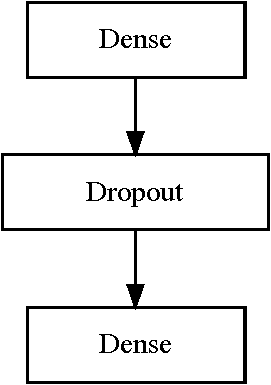
\includegraphics[scale=0.6]{graphics/text-classification/model.pdf}
% \end{wrapfigure}
\end{figure} 

Während dem Experiment wurde die optimale Grösse des Wörterbuchs durch Ausprobieren ermittelt. Das Bias ist bei den meisten der verwendeten Grössen des Wörterbuchs sehr gering. Der gewählte Ansatz scheint die Problemstellung bereits mit einem kleinen Vokabular gut bewältigen zu können.

Bei der Exploration der Grösse des Wörterbuchs wurde festgestellt, dass das Modell zur Klassifizierung mit einem grösseren Wörterbuch von 5'000 Wörtern die besten Ergebnisse, sprich die kleinste Varianz, liefert. Je grösser das Wörterbuch, desto schneller hat das Modell begonnen auswendig zu lernen (Overfitting). Um diesem Effekt entgegenzuwirken wurde ein grosser Dropout von 0.92 gewählt. Auch dieser Wert wurde explorativ ermittelt.

Bei dem gewählten Modell, mit einem Vokabular von 5'000 Wörtern und einem Dropout von 0.92, erreicht das Loss auf den Testdaten nach 23 Epochen Training den Wendepunkt (vgl. Abbildung \ref{text-class-results:val_loss}). Dabei wird eine Trefferquote von 98.4\% erzielt (vgl. Abbildung \ref{text-class-results:val_acc}). Zu diesem Zeitpunkt beginnt das Modell auswendig zu lernen. Es ist also nicht sinnvoll das Modell länger auf den vorliegenden Daten zu trainieren.

\begin{figure}[h!] 
  \captionsetup{width=.9\linewidth}
  \caption{Statistiken aus dem Training der Text-basierten Klassifizierung von Rechnungen}
  \label{text-class-results}
  \begin{subfigure}[b]{0.5\linewidth}
    \centering
    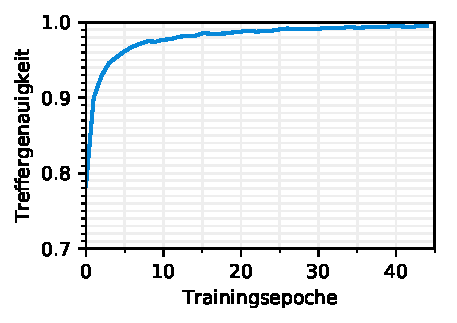
\includegraphics[scale=1]{graphics/matplot/textual-class__acc.pdf} 
    \caption{Trefferquote} 
    \label{text-class-results:val} 
    \vspace{2ex}
  \end{subfigure}%% 
  \begin{subfigure}[b]{0.5\linewidth}
    \centering
    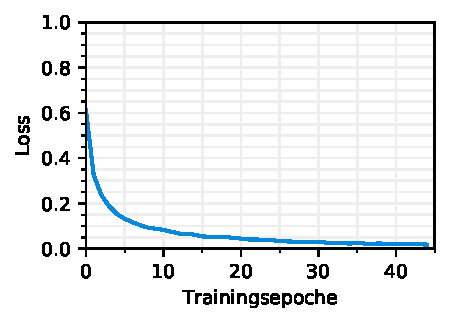
\includegraphics[scale=1]{graphics/matplot/textual-class__loss.pdf} 
    \caption{Loss} 
    \label{text-class-results:loss} 
    \vspace{2ex}
  \end{subfigure} 
  \begin{subfigure}[b]{0.5\linewidth}
    \centering
    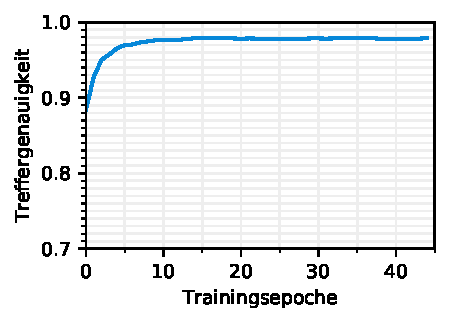
\includegraphics[scale=1]{graphics/matplot/textual-class__val_acc.pdf} 
    \caption{Trefferquote bei den Testdaten} 
    \label{text-class-results:val_acc} 
  \end{subfigure}%%
  \begin{subfigure}[b]{0.5\linewidth}
    \centering
    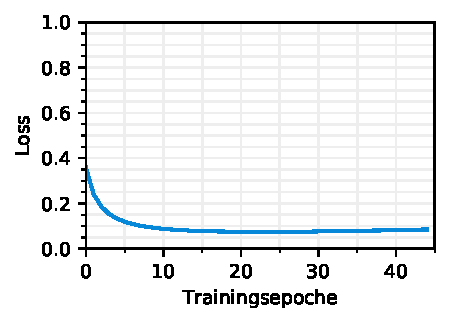
\includegraphics[scale=1]{graphics/matplot/textual-class__val_loss.pdf} 
    \caption{Loss bei den Testdaten} 
    \label{text-class-results:val_loss} 
  \end{subfigure}
  \centering
\end{figure}

Bei diesen guten Ergebnissen liegt es nahe, dass der Ansatz durch etwas Optimierung noch weiter verbessert werden kann. Im Folgenden wird eine Fehleranalyse, wie dies im Kapitel \ref{chap:error-analysis} beschrieben ist, gemacht. Zuerst wird aufgezeigt, worauf bei der Klassifizierung im vorliegenden Fallbeispiel besonders geachtet werden muss. Anschliessend werden aus den falsch klassifizierten Rechnungen Verbesserungsvorschläge abgeleitet. 

Die falsche Klassifizierung einer Rechnung ist vor allem dann problematisch, wenn diese einer Klasse zugewiesen wird, welche automatisch verarbeitet wird. Die Confusion Matrix in Abbildung \ref{text-classification-cm} zeigt, dass das Text-basierte Modell sechs aus 3'367 Rechnungen des Testsets fälschlicherweise als Fitness Rechnungen und fünf Rechnungen fälschlicherweise als Rechnungen für einen Sportverein klassifiziert hat. Diese Rechnungen würden automatisiert als solche abgerechnet werden, was der Kundin oder dem Kunden nicht vorenthalten bleibt. Die Kundin oder der Kunde müsste in diesem Fall aktiv werden, damit der Fehler bemerkt wird.

Würde eine Rechnung fälschlicherweise als Andere klassifiziert werden, so muss eine manuelle Verarbeitung der Rechnung stattfinden. In diesem Fall merkt die Kundin oder der Kunde nichts von dem Fehler. 

Aus den genannten Gründen ist die Genauigkeit für das vorliegende Beispiel die wichtigste Metrik. Die ermittelte Genauigkeit liegt bei 97.86\% (Fitness), 100\% (Optiker) respektive 96.50\% (Sportverein).

\begin{figure}[h!] 
%\begin{wrapfigure}{r}{0.5\textwidth} 
    \captionsetup{width=.9\linewidth}
    \caption{Confusion Matrix nach 23 Trainingsepochen des Text-basierten Modells zur Klassifizierung von Rechnungen}
    \label{text-classification-cm}
    \centering
    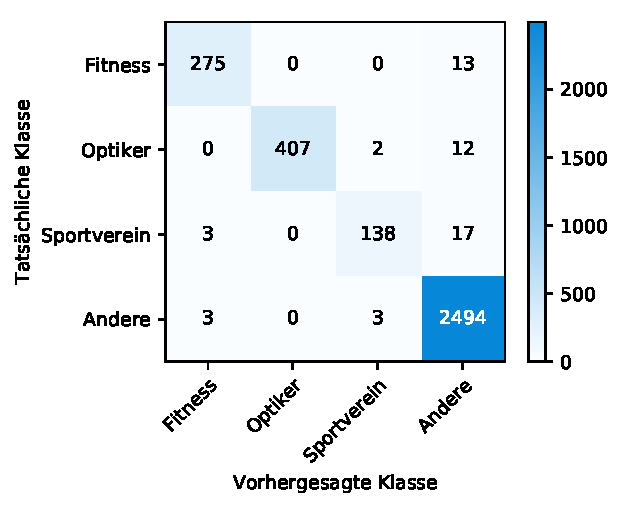
\includegraphics[scale=1]{graphics/matplot/textual-class__cm_22.pdf}
%\end{wrapfigure}
\end{figure}

% Im folgenden Kapitel wird Verbesserungspotential anhand einer Fehleranalyse für den präsentierten Ansatz aufgezeigt. Im Kapitel \ref{chap:class:conclusions} werden Schlussfolgerungen zur Rechnungsklassifizierung getroffen.

% \subsubsection{Verbesserungspotential der präsentierten Ansätze}

Die Insgesamt 53 falsch klassifizierten Rechnungen aus dem Testdatensatz sowie die während dem Training falsch klassifizierten Rechnungen wurden einer Fehleranalyse unterzogen. \textcite{MLYearning} suggerieren für die Verbesserung eines Modells dort anzusetzen, wo am meisten Falschklassifikationen vorliegen. Dabei wird argumentiert, dass dort das Potential, die Trefferquote zu erhöhen, am höchsten ist. In unserem Fall ist die Trefferquote aber eher nebensächlich. Die 42 fälschlicherweise als Andere klassifizierten Rechnungen haben keinen grossen negativen Einfluss auf den Geschäftsprozess. Aus diesem Grund fokussiert sich die Analyse auf die fälschlicherweise als eine der automatisierbaren Klassen klassifizierten Rechnungen. Während der Analyse wurden folgende Probleme und Verbesserungsmöglichkeiten identifiziert:

% TODO: this 4-th indentation is a bit shitty
\newpage

%{\parindent=0pt
%\textbf{Ungenauigkeiten des Optical Character Recognition}}

\label{chap:ocr-quality}
\textbf{Ungenauigkeiten des Optical Character Recognition}: Ein Problem, welches sofort ins Auge sticht, sind die Ergebnisse des Optical Character Recognition Systems. Diese sind teilweise sehr dürftig. Durch die mässige Qualität fotografierter Rechnungen können gewisse Wörter nur schlecht oder gar nicht erkannt werden. 

Durch diese Ungenauigkeiten während dem OCR Prozess entstehen viele Wörter mit Schreibfehlern. Das Wörterbuch erkennt aber nur Wörter, welche mit den gelernten Wörtern identisch sind. Wurde während dem Training des Wörterbuchs ein Wort nie in einer gewissen falschen Schreibweise angetroffen, so ist dieses Wort für das Klassifizierungsmodell nutzlos.

Eine Problematik für das Optical Character Recognition System ist eine schlechte Ausleuchtung des Fotos einer Rechnung. In diesem Fall erkennt das OCR System nur sehr wenig bis überhaupt kein Text. Dadurch kann die Rechnung nicht klassifiziert werden.

Eine weitere Problematik ist ein körniges Bild. In diesem Fall erkennt das OCR System diakritische Zeichen wie ein \textit{é}, wo keine sind. Dadurch kann ein Wort nicht im Wörterbuch gefunden werden und es trägt somit nicht zur Klassifizierung bei.

Um die Qualität der Resultate aus dem OCR System zu verbessern, stehen mehrere Optionen zur Verfügung. Als erstes sollte das Modell des OCR Systems, welches wie erwähnt selbst auch ein neuronales Netzwerk ist, auf den Rechnungen trainiert werden. Auch hier kommt das Konzept des Transfer Learning zum Einsatz. Das verwendete OCR System, Tesseract, erlaubt es nicht nur ganz eigene Modelle zu trainieren, sondern ermöglicht auch das Fine-tuning der mitgelieferten Modelle. In vorliegenden Fall würde ein Fine-tuning der mitgelieferten Modelle von Tesseract die Qualität der Ergebnisse womöglich stark verbessern, wie dies ein Beispiel im Tesseract Wiki suggeriert. Im Wiki wird erwähnt, dass das OCR Modell auf dem Modell bisher unbekannte Schriftarten trainiert werden sollte. Auch könnten durch das Fine-tuning einige Zeichen, welche Tesseract aktuell unbekannt sind, erlernt werden~\autocite{TesseractTraining}.

Im Wiki von Tesseract wird neben dem Fine-Tuning des OCR Modells auch die Aufbereitung der Bilder als zentraler Aspekt der Verbesserung der Qualität der OCR Resultate genannt. Unter der Aufbereitung versteht das Tesseract Wiki das Vergrössern, die Binärisierung, das Rotieren und Entzerren der Bilder sowie das Entfernen von Rauschen und dunkeln Rändern durch das Scanning~\autocite{TesseractQuality}.

In diesem Experiment ist die Grösse der vorliegenden Bilder kein Problem. Die meisten Bilder wurden in einer grossen Auflösung aufgenommen. Würde hier ein Problem vorliegen, so müsste beim digitalen Einreichen der Rechnungen über das Kundenportal, eine minimale Auflösung forciert werden.

Die Binärisierung, sprich das Umwandeln in Schwarz-Weiss-Bilder, der Rechnungen scheint durchaus ein Problem zu sein. Wie bereits erwähnt, sind die OCR Resultate dann besonders schlecht, wenn das Bild schlecht ausgeleuchtet ist. In diesem Fall ist der Binärisierungs-Algorithmus, welcher Tesseract standardmässig anwendet, nicht geeignet. Mit einem geeigneteren Algorithmus zur Binärisierung könnte die Qualität der OCR Ergebnisse verbessert werden. Die Bilder, welche in einem schlechten OCR Ergebnis resultieren, könnten durch verschiedene Binärisierungs-Algorithmen umgewandeln werden. Es kann dann jenes dieser umgewandelten Bilder verwendet werden, welches die besten OCR Resultate liefert.


Rotierte oder verzerrte Bilder sind im vorliegenden Experiment kein Problem. Die Rechnungen sind bereits richtig rotiert und kaum verzerrt.

Ein körniges Bild, ist wie erwähnt, aktuell ein Problem, welches die Qualität des OCR Ergebnis stark beeinflusst. Das Entfernen dieses Rauschens (Körnung) im Bild würde die Qualität des OCR Ergebnis und somit die Genauigkeit des Klassifizierungsmodells verbessern.

Scanning Rändern, wie diese auf dem Tesseract Wiki angemerkt werden, sind im vorliegenden Fall kein Problem. Ein ähnliches Problem, welches sich aber äussert, sind Ränder auf Fotografien von Rechnungen. Fotografiert jemand eine Rechnung, so ist meist noch etwas vom Hintergrund, beispielsweise einem Holztisch, zu sehen. Diese Ränder stören die Qualität der OCR Ergebnisse indirekt, durch eine verschlechterte Binärisierung, sowie direkt durch erkannte Buchstaben, wo eigentlich nur ein Hintergrund zu sehen ist. Es ist also zentral, diese Ränder zu entfernen. Viele Apps bieten bereits eine solche Funktion an, in welcher Ränder automatisch erkannt werden und der Nutzer die Möglichkeit hat, diese anzupassen. Eine solche Funktion ist für das vorliegende Fallbeispiel empfehlenswert.

Mit den genannten Ansätzen können die Resultate des OCR Systems verbessert werden. Es kann jedoch nicht davon ausgegangen werden, dass das OCR System immer alles korrekt erkennt. Aus diesem Grund ist eine Nachbearbeitung des OCR Resultates sinnvoll. Im Kapitel \ref{chap:grammar-correction} wurde ein Modell, basierend auf LSTM Netzwerken vorgestellt, welches darauf trainiert wird, Rechtschreibfehler zu korrigieren. Dieses Modell dürfte auch auf die Korrektur von OCR Fehlern anwendbar sein. Durch die Korrektur der OCR Fehler vor der Anwendung des Klassifizierungsmodells kann die Qualität dieses Modells erhöht werden. Mit einem Domain-Know-How basierten Ansatz zur Korrektur von Fehlern erreichen \textcite{OCRCorrection} eine knappe Verdoppelung der Qualität der Resultate aus dem OCR System. Selbst für qualitativ sehr schlechte Bilder erreichen werden sehr gute Resultate erreicht.

%{\parindent=0pt
%\textbf{Überrepräsentation einzelner Wörter in gewissen Klassen}}

\textbf{Überrepräsentation einzelner Wörter in gewissen Klassen}: Die Fielmann AG ist wohl einer der bekanntesten Optiker in der Schweiz. Sehen wir eine Rechnung und lesen Fielmann, denken wir sofort an eine Rechnung eines Optikers. Genau so scheint auch unser Modell zu denken, denn eine Rechnung von Fielmann wird stets als Rechnung von einem Optiker klassifiziert. Dies stellt aber ein Problem dar, denn Fielmann verkauft nicht nur Seh- sondern auch Hörhilfen.

Diese Problematik erinnert an das Problem der überrepräsentierten Klassen. Auf Stufe der Klassen trägt die Gewichtung der Loss-Funktion der Überrepräsentation einzelner Klassen Rechnung. Auf der Stufe des Vokabulars wird diesem Ungleichgewicht bisher keine Rechnung getragen.

Um diese Problematik zu lösen sind zwei Ansätze denkbar. Zum einen könnte das Wort Fielmann aus dem Wörterbuch ausgeschlossen werden. Dies könnte aber einen sehr negativen Einfluss auf die Klassifizierung tatsächlicher Rechnungen von Optikern haben. Zum anderen ist ein Over- oder Undersampling, also das künstliche vermehren oder vermindern, der Unter- beziehungsweise Überrepräsentierten Rechnungen denkbar. Das bedeutet, jene Fielmann Rechnungen welche Hörhilfen betreffen, sollten dem Modell während dem Training öfters vorgelegt werden. Damit würde das Modell auf diese Art von Rechnungen sensibilisiert werden.

%{\parindent=0pt
%\textbf{Nicht eindeutige Wahrscheinlichkeiten bei der Klassifizierung}}

\textbf{Nicht eindeutige Wahrscheinlichkeiten bei der Klassifizierung}: Die verwendete Methode der Klassifizierung verwendet vier Wahrscheinlichkeiten, mit welcher eine Rechnung einer bestimmten Klasse angehört. In Summe ergeben diese Wahrscheinlichkeiten immer 1. Die Klasse, bei welcher die Wahrscheinlichkeit am höchsten liegt, gewinnt. Es kann vorkommen, dass die Wahrscheinlichkeiten annähernd gleichmässig verteilt sind und eine Rechnung mit einer Klassen-Wahrscheinlichkeit von nur 25.1\% klassifiziert wird.

Um diese Problematik zu lösen, sollte eine minimale Wahrscheinlichkeit definiert werden, mit welcher eine Rechnung klassifiziert werden muss, damit das Ergebnis verwendet wird. Wahrscheinlichkeiten, welche unter diesem Minimum liegen, dürften nicht verwendet werden. Dieser Ansatz hat neben der Reduzierung der Fehlerquote aber auch eine Reduzierung der Automatisierung zur Folge. Es muss abgewogen werden, ob die AXA Gesundheitsvorsorge das Risiko einer höheren Fehlerquote eingehen möchte und dafür mehr Rechnungen automatisieren kann.

%{\parindent=0pt
%\textbf{Klassifizierung aufgrund irrelevanter Wörter}}

\textbf{Klassifizierung aufgrund irrelevanter Wörter}: Bei der Betrachtung einiger Rechnungen wurde festgestellt, dass diese hauptsächlich aus einem Einzahlungsschein bestehen. Dies kam besonders oft bei Sportvereinen vor. Aus diesem Grund assoziiert das Modell nun Wörter, welche auf dem orangen Einzahlungsschein vorkommen, mit einer Rechnung eines Sportvereins. Dies führt dazu, dass Rechnungen, mit orangem Einzahlungsschein und keinen anderen klaren Indikatoren, fälschlicherweise als Rechnung eines Sportvereins klassifiziert werden.

Diese Problematik lässt sich durch ein sogenanntes Blacklisting der Wörter, welche auf dem Orangen Einzahlungsschein vorkommen, lösen. Dabei dürfen aber nicht nur die exakten Wörter herausgefiltert werden. Auch ähnliche Wörter, sprich Wörter mit Schreib- bezeiehungsweise OCR-Fehlern müssten gefiltert werden.

%{\parindent=0pt
%\textbf{Limitierung auf bekannte Wörter}}

\textbf{Limitierung auf bekannte Wörter}: Das angewendete Verfahren zum Word embedding, basieren auf einem Wörterbuch, funktioniert nur für bekannte Wörter. Wörter mit einem Tippfehler oder Synonyme können aufgrund dem fehlenden Embedding nicht zur Klassifizierung beitragen.

Anstelle des aktuell verwendeten, einfachen Word Tokenizer könnte ein komplexeres Word embedding (vgl. Kapitel \ref{chap:embedding}) angewendet werden. Wie bereits im Kapitel \ref{chap:transfer-learning} erwähnt, zeigen jüngste Forschungen, dass auch in diesem Bereich dank Transfer Learning mit nur wenig Datensätzen gute Ergebnisse erzielt werden können. Das im Oktober 2018 publizierte BERT Modell verspricht in diesem Bereich eine revolutionäre Verbesserung. Das Modell könnte in diesem Fall als Grundlage für das Transfer Learning dienen~\autocite{Devlin2018}.
